
\section{Extended Structural Balance Theory (ESBT)} \label{sec:esbt}
In this section, we introduce a new and more fine-tuned way to define
structural balance that we will call extended structural balance
theory, or ESBT for short. The psychological explanation for weak
structural balance relies on the concept of stress. Certain situations
cause stress in interactions and as a result, are not considered
natural. So, in balanced situations such stress must not exist. We
define this stress more precisely as a function of the strength of
relationships.

In classical balance theory, relations are restricted to binary values
($+$/$-$), which we interpret as trust and distrust. When Cartwright
and Harrary first formalized the theory of structural balance, they
also suggested that relationships of interest exist in varying
degrees, and that their theory is built on the incomplete
representation of strengths of relations~\cite{Cartwright:56}. Tie
strength is a well-studied concept in social psychology. A person may
have close friends and acquaintances (strong/weak ties), with
different trust expectations. A strong tie may represent a trust
relation corresponding constructs relevant to high risk situations,
while a weak tie may be trusted for low risk situations like providing
private information~\cite{Granovetter:1973}.

To model this distinction, we consider a scenario where relationships
have varying strengths. A strong positive link represents a close
friendship or family tie, i.e. strong trust constructs, and a strong
negative link represents hatred, i.e. strong distrust
constructs. However, many other types of trust relationships may exist
in between the spectrum of (strong) trust and (strong) distrust. For
example, a negative bias may be considered a weak distrust and a weak
tie may represent weak (positive) trust.
 
A complete balance theory should be able to deal with relationhips
with strengths.  As a first step, we need to have a measurement of
relations with various strengths. While it is arguable whether
such strengths can be expressed by numerical values, it is fairly
clear that the strength of any two relations can be compared. For
positive relations such as liking, valuing or approving, two
relationships are comparable in terms of which one is stronger than
the other. Similar argument applies to two negative
relations. Finally, a positive relation and a negative relation are
comparable by their signs. Hence, relations with strengths by nature
inherit a total ordering.
 
Let the collection of relations with strengths be $E$. An edge $(A,B)$
and a relation with associated strength $e$ will be used
interchangeably in later discussion. We pick the ordering $\preceq$
such that, $e_{1} \preceq e_{2}$ denotes $e_{1}$ is positively
equivalent to or stronger than (or negatively equivalent to or weaker
than resp.) $e_{2}$. That is, if $e_{1}, e_{2}$ are both positive
relations, $e_{1} \preceq e_{2}$ if $e_{1}$ is at least as positive as
$e_{2}$ in terms of strengths; if $e_{1}, e_{2}$ are both negative
relations, $e_{1} \preceq e_{2}$ if $e_{1}$ is at most as negative as
$e_{2}$ in terms of strengths; if $e_{1}, e_{2}$ are of different
signs, $e_{1} \preceq e_{2}$ if $e_{1}$ is positive and $e_{2}$ is
negative. In the simplest case where we have only positive and
negative relations, we have that $+ \preceq -$. 
 
We also consider a {\bf neutral relationship} as one that is unbiased,
which will be denoted as $O$. Basically a neutral relationship is a
non-negative and non-positive relationship, corresponding to no
opinion and no bias. In the case of incomplete networks,  classic balance theory implicitly considered two types of triads with
neutral relations balanced: ``$+, +, O$",
``$+,-,O$"~\cite{kleinberg-book}. With the introduction of neutral
relations, $E$ can be partitioned into three subsets: positive
relationships $P$, negative relations $N$ and neutral relations
$O$. Following the definition of ordering $\preceq$, it is clear that
for any $e_{+} \in P$, $e_{O} \in O$, $e_{-} \in N$, $e_{+} \preceq
e_{O} \preceq e_{-}$ holds. We use $\tuple{e_1}{e_2}$ to denote the
set of relations $\tuple{e_1}{e_2}$ = $\{e\:\mid\: e_1\preceq e\preceq
e2\}$. Hence, given $\tuple{e_1}{e_2}$, the lower bound $e_1$
represents the strongest possible relationship and the upper bound
represents $e_2$ represents the weakest possible relationship in this
range.
 
\subsection{Principles of Structural Balance}
A triad is the smallest unit in balance theory, within which two of
its relations cause influence over the third one.  Such an influence
will limit the range of comfortable relations of the third relation in
a balanced state; and if it goes out of range, tension occurs and
participants will suffer from {\bf stress}. Participants will seek
relationship changes to resolve this type of stress. We call such range
of relations {\bf tolerance}, with which we interpret structural
balance at a finer level.

Given a network of nodes $G=(V,E)$, there exists a tolerance for each
pair $(A,B)$ of nodes of the form $\tuple{e_1}{e_2}$ which is
constrained by the triads $(A,B)$ is part of. When there is no
constraint, i.e. stress, on a specific relationship, the tolerance
includes any relationship in $E$. We propose two principles regarding
tolerance: transitivity and heterophily.

\begin{principle}[Transitivity of positive relationships]
Let individuals $A$, $B$, $C$ in a network form a traid, and $(A,B)$,
$(A,B)^{'}$, $(B,C)$ be positive. Suppose $T=\tuple{e_1}{e_2}$ denotes
the tolerance of $(A,C)$ based on relations $(A,B),(B,C)$, and
$T'=\tuple{e_1'}{e_2'}$ denotes the tolerance based on
$(A,B)^{'},(B,C)$. If $(A,B)' \preceq (A,B)$ then we have that
$e_2'\preceq e_2$.

Furthermore, there exists a $e_{sp} \in P$ such that if $(A,B)\preceq
e_{sp}$ and $(B,C) \preceq e_{sp}$, then $e_{2} \preceq e_{O}$ holds
for all $e_{O} \in O$. That is, $T$ will only have positive relations
beyond a certain threshold $e_{sp}$.
\end{principle}
In other words, the fact that B are friends with both A and C provides
the freedom for $A$ and $C$ to become friends; and there is stress on
$A$ and $C$ to get close. The stronger the relation between $(A,B)$
and $(B,C)$, the higher the stress between $(A,C)$ to be connected
(more) positively, and the resulting tolerance is restricted to be
more positive.

The stress that is based on positive relations has been frequently
defined by SBT and WSBT. Positive relations in a triad cause stress
for the remaining relations to be positive. As a result, both in SBT
and WSBT, a balanced network consists of communities that are
connected to each other with positive ties. When we consider the
strength of relations, we generalize this by saying that the more
positive two of the relations are in a tie, there is lesser tolerance
for negative trust values.

There is a point when the strength of the two positive relations are
strong enough such that it is imbalanced for $(A,C)$ to remain
unfriended, i.e. neutral. This observation is inspired by the ``strong
triadic closure" in~\cite{kleinberg-book}. In trust literature, it is
often referred as the ``transitivity of trust'' though transitivity is
also used in other contexts.

\begin{principle} [Heterophily in relationships] 
Let individuals $A$, $B$, $C$ in a network form a triad. Suppose
$T=\tuple{e_1}{e_2}$ denotes the tolerance of $(A,C)$ based on
relations $(A,B),(B,C)$, and $T'=\tuple{e_1'}{e_2'}$ denotes the
tolerance based on $(A,B)^{'},(B,C)$. We have that if
$(A,B)' \preceq (A,B) \preceq (B,C)$, or $ (B,C) \preceq (A,B) \preceq
(A,B)'$, then $e_1\preceq e_1'$.

Furthermore, suppose there is a well-defined concept of difference
between two relations with strengths. Then, the larger difference
between $(A,B)$ and $(B,C)$ is, less positive $e_1$ (the lower bound)
is.
\end{principle}
Given individuals $A$, $B$, $C$ in a network, if the relationship
between $(A,B)$ and the relation between $(B,C)$ differs to some
extent, then the tolerance is geared towards the
negative. Furthermore, the more different the strength of the
relationships are, the tolerance is geared towards more
negative values. 

The second type of stress is an interpretation of homophily. We note
that homophily, i.e. having common friends or enemies, may sometimes
cause stress (in $+,+,+$) but sometimes it does not (in $-,-,-$ for
WSBT). However, lack of homophily, which we call heterophily does
cause stress. For example, consider the case $+,+,-$ for $(A,B)$,
$(B,C)$ and $(A,C)$. There is stress on $(A,C)$ to be positive due to
transitivity. But, there is also stress on $(A,B)$ and $(B,C)$ to be
negative. Either way, the result will be more desirable: either all
being friends, or having two friends with a common enemy. We call the
second type of stress the principle of heterophily. The more different
the ties are (the strongest difference is between distrust and trust,
and the weakest difference is between two identical trust ties), the
more pressure there is for the tie to be negative.  At a point when
the difference between $(A,B)$ and $(B,C)$ is significant enough, we
argue that a positive value for $(A,C)$ will cause imbalance. This is
inspired by the observation that two people who have severely
conflicted relationships with a common neighbor, e.g., one is the
other's close friend's enemy, are not likely to be friends.

\begin{table}[h]
\begin{center}
 \begin{tabular}{cc|cl} 
  $(A,B)$ & $(A,C)$ & Tolerance for $(B,C)$ &  \\ \hline
  $+$ & $+$ & $\tuple{+}{O}$ & Transitivity \\
  $+$ & $-$ & $\tuple{O}{-}$ & Heterophily \\ 
  $-$ & $-$ & $\tuple{+}{-}$ & No stress \\ 
 \end{tabular}\\  \vspace{1mm}
\caption{\label{ref:classic_balance}Tolerance rules in structural balance theory}
\end{center}
\end{table}

The two principles help interpret balance in terms of relations with
strengths precisely. A triad is balanced if all relationship strengths
are within the tolerance implied by the other relationships in the
triad.

\begin{definition} [Balance]
A triad $A,B,C$ is balanced if for all pairs $(A,B)$, given the
tolerance $\tuple{e_1}{e_2}$ of $(A,B)$ with respect to $(B,C),(A,C)$,
we have that $(A,B)\in \tuple{e_1}{e_2}$. 
Given a network $G$ of relationships, $G$ is said to be balanced if
for all triads in the network are balanced.
\end{definition}

The tolerance rules for the Davis's balance theory are
given in Table~\ref{ref:classic_balance}. Notice that neutral
relations ``$O$" are also added. This is because triangles ``$+, +,
O$" and ``$+, -, O$" are allowed implicitly in their theory in the
general case of incomplete graphs. According to the table, triads (1), (2) and
(3) from Figure~\ref{fig:balance_strong} are balanced as each relation
strength is within the tolerance, but triad (4) is not
balanced. Hence, our theory generalizes WSBT in the
classical balance theory.

\subsection{Balance theorems with weak and strong ties.} \label{sec:weak_strong}
In this section, we show how our reasoning can be applied to a network
with multiple types of relationships. We consider a set of discrete
labels (shown in Table~\ref{ref:rel_types}) that have been discussed
in previous literature and show that we can reason about balance in
such a network using our two principles. 

{\bf Strong positive ties, s+ (trust)} are similar to a close
friendship. There is a strong expectation of reciprocity, similarity
of tastes (homophily), common intentions and benevolence towards each
other~\cite{Tomasello:2005}. The traditional definition of SBT is
based on these types of positive relationships.

{\bf Strong negative ties, s- (distrust)} are generally explained as
having negative experiences with someone which is indicative of their
negative intentions, unreliability and overall belonging to groups
that are not considered trustworthy~\cite{Fiske:2007}. Even when a
distrusted person behaves in a trustworthy way, this could be
considered a trick to get one to trust them.

\begin{table} [htbp!]
\begin{center}
\begin{tabular}{p{1.6in}p{1.6in} }
Relation Type & Interpretation \\ \hline
Strongly positive (s+) & close friendship, trust  \\ 
Weakly positive (w+) & aquiantance \\
Neutral (O) & unbiased relation, no relation  \\
Weakly negative (w-) & minor disagreement, negative bias  \\
Strongly negative (s-) & hatred, distrust  
\end{tabular}\\\vspace{1mm}
\caption{\label{ref:rel_types}Strength of relations: $s+\preceq w+\preceq O\preceq w- \preceq s-$.}
\end{center}
\end{table}

However, these are not all the different classes of relationships that
one might consider in a network. While one might consider a continuum
of tie strength, we summarize some additional discrete classes. {\bf
  Weak positive ties, w+ (weak trust)} can be considered a utilitarian
type of trust. Interacting with someone who is only trusted partially is
more risky, but can be acceptable in certain situations. For example,
Uzzi~\cite{Uzzi:1996} uses the term embedded vs. arm's length ties to
distinguish between the two types of trust. While a close friend is
highly trusted, they may not have access to the resources a more risky
contact may provide. Granovetter~\cite{Granovetter:1973} uses the term
weak tie to talk about a relationship that is an acquaintance, not a
close friend. Weak ties give access to less privileged information
than strong ties, but come from outside of one's close network. In
both cases, there is a trust relationship between two people, but this
does not imply a continuous interaction or a strong affective
component as in trust.

We also introduce {\bf weak negative ties, w- (weak distrust)} to
model cases in which there is a certain amount of distrust as a result
of biases stemming from social groups people belong to or heresay that
may not be as strong as distrust~\cite{Ames:2011}. In essence, the
burden of proof of one's trustworthiness is much higher in distrust
than in weak distrust, but in both cases, positive evidence is not
evaluated in the same way as in trusting relations. These five types
of relationships are summarized in Table~\ref{ref:rel_types}.


\begin{table}[htbp!]
\begin{tabular}{p{1.6in}|p{1.2in}}
 \begin{tabular}{p{0.3in}p{0.3in}p{0.5in}} 
$(A,B)$ & $(A,C)$ & $(B,C)$'s tolerance \\ \hline
$s+$ & $s+$ & $\tuple{s+}{w+}$ \\
$s+$ & $w+$ & $\tuple{s+}{O}$  \\
$s+$ & O & $\tuple{s+}{w-}$ \\
$s+$ & $w-$ & $\tuple{O}{s-}$ \\ 
$s+$ & $s-$ &   $\tuple{w-}{s-}$ \\
$w+$ & $w+$ & $\tuple{s+}{w-}$ \\
$w+$ & O & $\tuple{s+}{s-}$ \\
& & 
\end{tabular} &
\begin{tabular}{p{0.3in}p{0.3in}p{0.5in}} 
$(A,B)$ & $(A,C)$ & $(B,C)$'s tolerance \\ \hline
$w+$ & $w-$ & $\tuple{w+}{s-}$ \\
$w+$ & $s-$ & $\tuple{O}{s-}$ \\ 
O & O & $\tuple{s+}{s-}$ \\ 
O & $w-$ & $\tuple{s+}{s-}$ \\ 
O & $s-$ &  $\tuple{w+}{s-}$ \\ 
$w-$ & $w-$ & $\tuple{s+}{s-}$ \\ 
$w-$ & $s-$ & $\tuple{s+}{s-}$ \\ 
$s-$ & $s-$ & $\tuple{s+}{s-}$ \\
\end{tabular}
\end{tabular} \\\vspace{1mm} 
\caption{\label{tab:weak_strong_tolerance}Tolerance of strong, weak \& neutral relations}
\end{table}

Given these relationship types, we now describe the tolerance for
different triads in Table~\ref{tab:weak_strong_tolerance} and the
resulting imbalanced triads or structures in
Table~\ref{tab:imbalanced_extended}. Notice that the triads with
two positive relations and one negative relation are imbalanced as
they are in classic balance theory, except for the cases in which all
three relations as weak. In fact, the types of triads that consist
of weak relations and neutral relations only are not considered to be
imbalanced structures. The argument here is that when all relations
are weak or neutral, the influence inside the triad is not significant
enough to draw tension. Also, triads of type ``$s+$ $s+$ O" and
``$s+$ $s-$ O" are considered to be imbalanced structures. The
arguments against each type of imbalanced structure is listed in
Table~\ref{tab:imbalanced_extended}.

\begin{table}[htbp!]
\begin{center}
 \begin{tabular}{p{3in}}
Triads and  the argument for stress \\ \hline
$(s+ s+ s-)$ $(s+ s+ w-)$ $(s+ w+ s-)$ $(s+ w+ s-)$ $(w+ w+ s-):$ \\
my two friends cannot get along with each other \\ \\

$(s+ s+ O)$: my two close friends do not friend each other \\ 
$(s+ s- O)$: my enemy's close friend does not pick a side\\ 
\end{tabular} \vspace{4mm}
\caption{\label{tab:imbalanced_extended}Imbalanced triadic structures
  in the presence of strong and weak ties.} 
\end{center}
\end{table}
\vspace*{0in}

\subsection{Relation Distance and General Expression of Balance}
The concept of extended balance is meaningful only if the tolerance
rules can be explicitly defined, so that whether a triad and a network
is balanced or not can be determined. Whenever relations
are drawn from a finite and small set, this is easy to do. However, it
is considerably more complex in the general case when the strengths
of relations are drawn from arbitrary numerical values. 

To handle such cases, we refine the measurement of relations with
strengths from a total ordering to positive real values. In
particular, we define function $\psi: E \rightarrow R^{+}$ such that,
for two relations $e_{1}, e_{2} \in E$, $\psi(e_{1}) \leq \psi(e_{2})$
if and only if $e_{1} \preceq e_{2}$.  Since positive values can be
seen as metric distances, we call $\psi(e)$ the relation distance of
$e$.  In other words, relations with varying strengths are represented
by distances with different lengths.  More negative strengths are
represented by larger distances and more positive strengths are
represented by smaller distances. We propose the following general
rule of tolerance with the concept of relation distance.


%% In the case of WSBT, Table 1 set up
%% such tolerance rules. In the extended case when strong/weak ties are
%% introduced, Table 3 provides the tolerance rules. For general cases
%% when relation strengths are not limited to particular types, however,
%% the tolerance rules are not defined. We address this problem by
%% expressing relation in terms of metric distance, based on which we set
%% up a uniform tolerance rule that generalizes Table 1 and 3.

%% In previous discussion, relations are measured by a complete
%% ordering. To express it as distance, we need an additional assumption
%% that the difference between any two relation strengths are well
%% defined. We introduce a function from relation to real values: $\psi:
%% E \rightarrow R^{+}$. For each relation $e \in E$, $\psi(e)$ denotes
%% its distance expression, which will be called relation distance for
%% simplicity. The ordering relation is then reduced to the numerical
%% comparing operator $<$.  In particular, $\psi(e_{1}) < \psi(e_{2})$ if
%% and only if $e_{1} \preceq e_{2}$.


\begin{definition} \label{def:gen_tolerance}
Given adjacent relations $(A,B)$ and $(B,C)$, the tolerance of $(A,C)$
is given by $[|\psi(A,B)-\psi(B,C)|, \psi(A,B)+\psi(B,C)]$.
\end{definition}

It can be easily checked that the general tolerance rule agrees with
Principle 1 and 2 by substituting $\leq$ for $\preceq$.  Immediately, we have the following
theorem.
\begin{theorem} 
Given a triad $(A,B,C)$, if $\psi(A,B)$, $\psi(B,C)$, $\psi(A,C)$
satisfies the metric triangle inequality, then $(A,B,C)$ is balanced.
\end{theorem}

To illustrate how the distances can be used to represent a given set
of strength values, we revisit WSBT. Consider two thresholds:
$b_{+} < b_{-}$ such that if $\psi(e)\geq b_{-}$ then the relationship
$e$ is negative. Similarly, if $\psi(e)\leq b_{+}$, then $e$ is
a positive relationship. For any value $b_{+} < \psi(e) < b_{-}$, the
relationship is considered neutral. We can see that as long as
$b_{-}>2b_{+}$, Table~\ref{ref:classic_balance} is equivalent to
Definition~\ref{def:gen_tolerance}.

\begin{figure}[th]
\centering
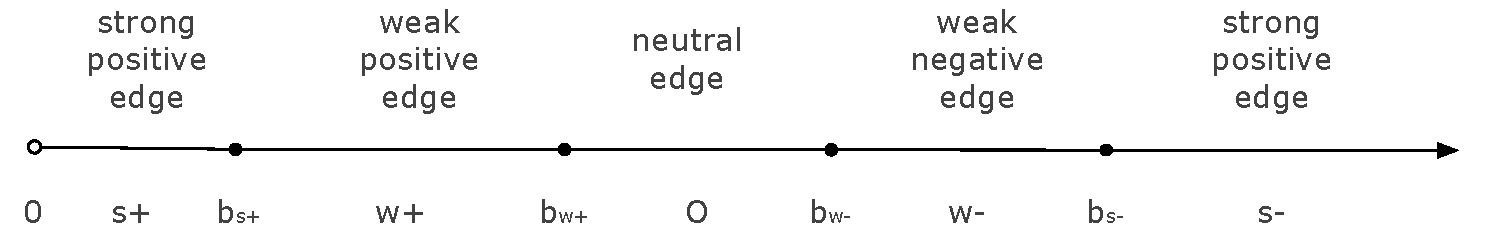
\includegraphics[height=0.55in]{Figs/mapping2.pdf}
\vspace*{-0.1in}
\caption{\label{fig:partition}Partitioning of distances:
  $(0,b_{s+}]:s+$, $(b_{s+}, b_{w+}): w-$, $[b_{w+}, b_{w-}]:O$,
$(b_{w-}, b_{s-}):w-$, and $ [b_{s-}, \infty):w+$.}

\end{figure}

Similarly, to capture the example from Section~\ref{sec:weak_strong},
we consider the partitioning of the distance domain given in
Figure~\ref{fig:partition}. We can see that if the following
conditions are satisfied for the boundary parameters: 

\begin{tabular}{p{1.5in}p{1in}}
$b_{w+}  > 2b_{s+}$ & $b_{s-}  > b_{w-} + b_{s+}$  \\
$b_{s-}  > 2b_{w+}$ & $b_{w-}  > b_{w+}+b_{s+}$
\end{tabular} 

\noindent the tolerance given in
Table~\ref{tab:weak_strong_tolerance} are equivalent to
Definition~\ref{def:gen_tolerance}, and all triads shown in
Table~\ref{tab:imbalanced_extended} are imbalanced according to metric triangle
inequality.
